\documentclass[aspectratio=169,11pt]{beamer}
\usetheme{Madrid}
\usepackage{graphicx}
\usepackage{booktabs}
\usepackage{tikz}
\usetikzlibrary{arrows.meta,positioning}
\graphicspath{{figures/}}

% ---- colours ----------------------------------------------------------
\definecolor{ink}{HTML}{14213D}
\definecolor{fallc}{HTML}{B8481F}
\definecolor{adlc}{HTML}{1F5F99}
\definecolor{paper}{HTML}{F5F3EC}
\setbeamercolor{palette primary}{bg=ink,fg=white}
\setbeamercolor{palette secondary}{bg=ink!85,fg=white}
\setbeamercolor{palette tertiary}{bg=ink!70,fg=white}
\setbeamercolor{title}{bg=ink,fg=white}
\setbeamercolor{frametitle}{bg=ink,fg=white}
\setbeamercolor{structure}{fg=adlc}
\setbeamercolor{block title}{bg=adlc,fg=white}
\setbeamercolor{block body}{bg=adlc!10,fg=black}
\setbeamercolor{alerted text}{fg=fallc}
\setbeamertemplate{navigation symbols}{}
\setbeamertemplate{itemize items}[circle]

\title[Early-Warning Fall Prediction]{Early-Warning Fall Prediction for Assistive Robotics}
\subtitle{A cost-sensitive, time-to-impact trade-off analysis on UMAFall}
\author[{Sujal Chaudhari}]{{Sujal Chaudhari} \,$\cdot$\, {IS24BM005}}
\institute[PRML]{Pattern Recognition and Machine Learning (PRML) -- course project\\{Interdisciplinary sciences, IIT Dharwad}}
\date{November 2026}

\newcommand{\tmark}{$\tau$}

\begin{document}

\begin{frame}[plain]
\titlepage
\end{frame}

% ----------------------------------------------------------------------
\begin{frame}{The problem: a fall alarm after the fall is too late}
\begin{columns}[T]
\begin{column}{0.58\textwidth}
\begin{itemize}\setlength\itemsep{0.9em}
\item Falls are a leading cause of injury-related death and hospitalisation after age 65, and a safety risk for humanoid and assistive robots.
\item \textbf{Detection} reports a fall when the person is already on the floor.
\item \textbf{Prediction} must act in the few hundred milliseconds between losing balance and impact, when an airbag, a robot gait correction or an alert can still help.
\end{itemize}
\end{column}
\begin{column}{0.4\textwidth}
\begin{block}{My question}
How early can a wearable-sensor classifier warn, and what does extra lead time cost?
\end{block}
\begin{itemize}
\item Lead time $\tau$ before impact
\item Missed falls
\item False alarms
\end{itemize}
\end{column}
\end{columns}
\end{frame}

% ----------------------------------------------------------------------
\begin{frame}{What is new in this project}
\small
\begin{enumerate}\setlength\itemsep{0.55em}
\item \textbf{Time-to-impact formulation:} the target is relabelled for every lead time $\tau$ (positive, negative and ambiguous zones), with strictly causal windows, so detection ($\tau=0$) and early warning ($\tau>0$) share one framework.
\item \textbf{Leakage-safe cost-sensitive alarm:} the threshold minimises $C_{FN}\cdot FN + C_{FP}\cdot FP$ on training subjects only (nested), with a sweep of the cost ratio.
\item \textbf{Event-level evaluation:} falls caught early, warning time and false alarms per minute, not just accuracy.
\item \textbf{Metric audit and decision layer:} a \emph{strict} trial metric and temporal persistence of the score, reported with their limited benefit.
\item \textbf{Live streaming demo} that replays any trial window by window.
\end{enumerate}
\vspace{0.3em}
\begin{alertblock}{Not claimed}
No new classifier: the models are standard; the contribution is the problem formulation, evaluation protocol and decision analysis.
\end{alertblock}
\end{frame}

% ----------------------------------------------------------------------
\begin{frame}{Dataset: UMAFall (Universidad de M\'alaga)}
\small Source: ``UMAFall: Fall Detection Dataset'', public on figshare, doi 10.6084/m9.figshare.4214283.
\vspace{0.4em}

\begin{center}
\begin{tabular}{cccc}
\textcolor{fallc}{\Huge 746} & \textcolor{fallc}{\Huge 208} & \textcolor{adlc}{\Huge 538} & \textcolor{adlc}{\Huge 19}\\
trials (15\,s each) & simulated falls & daily activities & volunteers
\end{tabular}
\end{center}
\vspace{0.3em}
\begin{columns}[T]
\begin{column}{0.49\textwidth}
\textbf{Sensors}
\begin{itemize}\small
\item 5 positions: chest, waist, wrist, ankle, smartphone in right pocket
\item Tags: accelerometer + gyroscope (+ magnetometer), $\approx$20\,Hz
\item Phone: accelerometer only, $\approx$200\,Hz
\end{itemize}
\end{column}
\begin{column}{0.49\textwidth}
\textbf{Activities}
\begin{itemize}\small
\item \alert{Falls:} forward (71), backward (73), lateral (64)
\item \textcolor{adlc}{ADLs:} walking, jogging, hopping, bending, sitting, lying down, stairs, clapping, door, phone call, hands up
\item Vigorous ADLs are deliberate \emph{hard negatives}
\end{itemize}
\end{column}
\end{columns}
\end{frame}

% ----------------------------------------------------------------------
\begin{frame}{What a fall looks like in the signal}
\begin{columns}[c]
\begin{column}{0.52\textwidth}
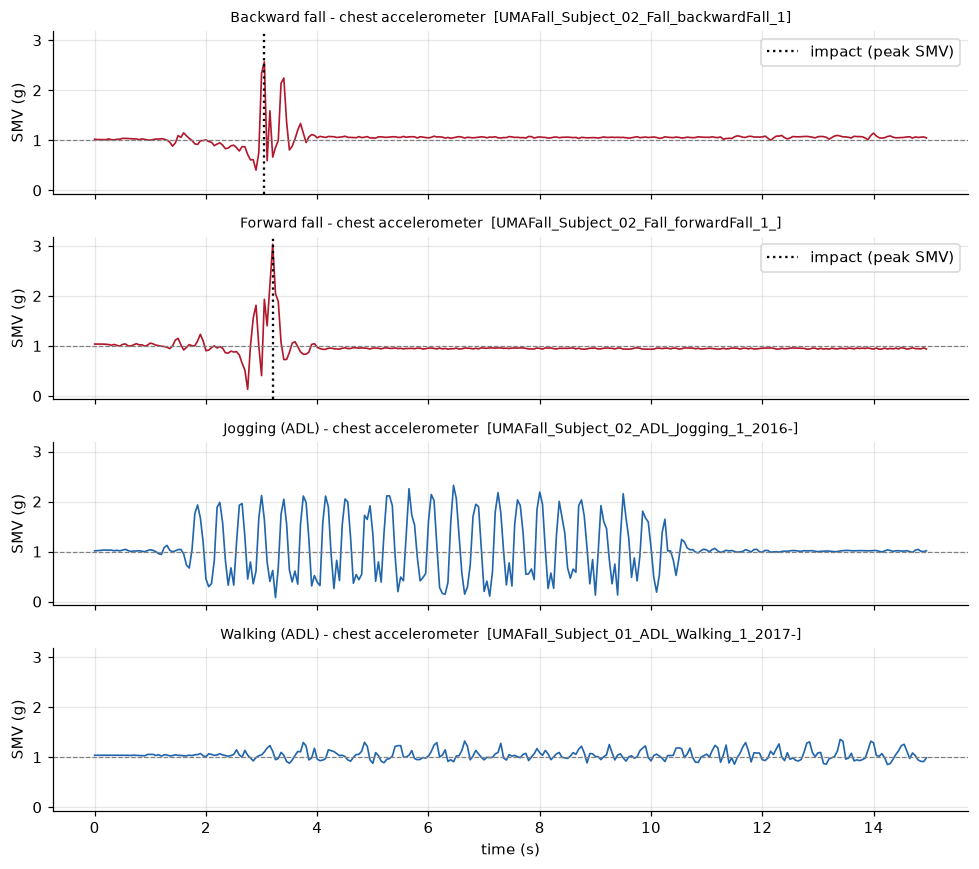
\includegraphics[width=\textwidth,height=0.78\textheight,keepaspectratio]{fig01_signals.png}
\end{column}
\begin{column}{0.46\textwidth}
\small
\begin{enumerate}\setlength\itemsep{0.5em}
\item \textbf{Rest:} SMV $\approx$ 1\,g (body supported)
\item \alert{\textbf{Free-fall dip:}} support vanishes, SMV $\to$ 0\,g \emph{before} impact: the early-warning cue
\item \textbf{Impact spike:} sharp peak at the ground
\item \textbf{Stillness:} flat signal, too late to warn
\end{enumerate}
\vspace{0.4em}
$\mathrm{SMV}=\sqrt{x^2+y^2+z^2}$ is orientation-invariant.\\[0.4em]
Jogging reaches peaks as high as a fall.
\end{column}
\end{columns}
\end{frame}

% ----------------------------------------------------------------------
\begin{frame}{Workflow: from raw CSV files to a cost-aware alarm}
\centering
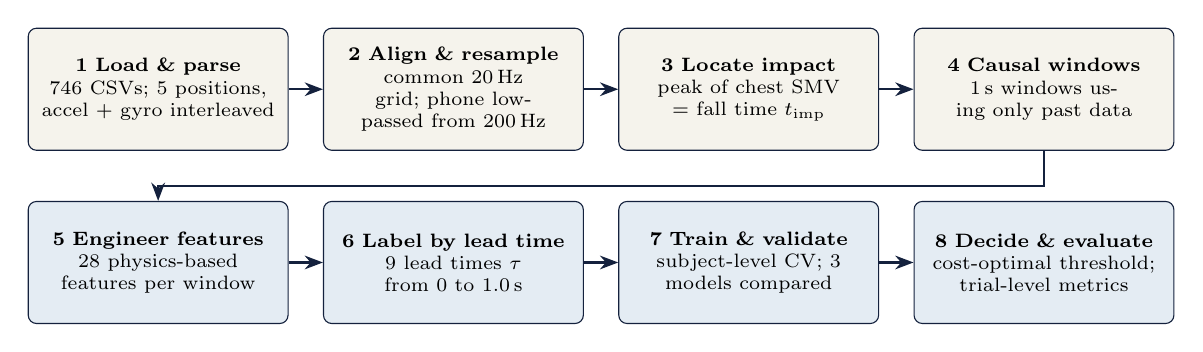
\begin{tikzpicture}[
  box/.style={draw=ink,rounded corners=3pt,fill=paper,minimum width=3.3cm,minimum height=1.55cm,text width=3.0cm,align=center,font=\scriptsize},
  arr/.style={-{Stealth},thick,ink}]
\node[box] (a) at (0,0)    {\textbf{1 Load \& parse}\\746 CSVs; 5 positions, accel + gyro interleaved};
\node[box] (b) at (3.75,0) {\textbf{2 Align \& resample}\\common 20\,Hz grid; phone low-passed from 200\,Hz};
\node[box] (c) at (7.5,0)  {\textbf{3 Locate impact}\\peak of chest SMV = fall time $t_{\mathrm{imp}}$};
\node[box] (d) at (11.25,0){\textbf{4 Causal windows}\\1\,s windows using only past data};
\node[box,fill=adlc!12] (e) at (0,-2.2)    {\textbf{5 Engineer features}\\28 physics-based features per window};
\node[box,fill=adlc!12] (f) at (3.75,-2.2) {\textbf{6 Label by lead time}\\9 lead times $\tau$ from 0 to 1.0\,s};
\node[box,fill=adlc!12] (g) at (7.5,-2.2)  {\textbf{7 Train \& validate}\\subject-level CV; 3 models compared};
\node[box,fill=adlc!12] (h) at (11.25,-2.2){\textbf{8 Decide \& evaluate}\\cost-optimal threshold; trial-level metrics};
\draw[arr] (a)--(b); \draw[arr] (b)--(c); \draw[arr] (c)--(d);
\draw[arr] (d.south) -- ++(0,-0.45) -| (e.north);
\draw[arr] (e)--(f); \draw[arr] (f)--(g); \draw[arr] (g)--(h);
\end{tikzpicture}
\end{frame}

% ----------------------------------------------------------------------
\begin{frame}{Preprocessing: data problems found, and what I did}
\small
\begin{tabular}{@{}p{0.46\textwidth}p{0.48\textwidth}@{}}
\toprule
\textbf{Found in the data} & \textbf{What I did}\\
\midrule
Phone logs accelerometer only at $\approx$200\,Hz; tags log 3 sensors at $\approx$20\,Hz & Block-averaged and resampled the phone to 20\,Hz; magnetometer left out\\[0.7em]
TimeStamp repeats for 2--3 rows (coarse clock) & Fitted a line of timestamp vs.\ sample index: evenly spaced time axis\\[0.7em]
Sensors missing in some trials (waist 617, ankle 643, chest 745 of 746) & Never assume 5 sensors; chest is the main position, others compared on the trials that have them\\[0.7em]
4 fall trials peak below 1.5\,g; impact time ranges 1.9--14.6\,s & Impact = peak SMV; all trials kept, listed as a limitation\\
\bottomrule
\end{tabular}
\end{frame}

% ----------------------------------------------------------------------
\begin{frame}{Feature engineering: 28 features tied to the physics}
\small
\begin{tabular}{@{}p{0.2\textwidth}p{0.4\textwidth}p{0.32\textwidth}@{}}
\toprule
\textbf{Group} & \textbf{Examples} & \textbf{Why}\\
\midrule
\alert{Free-fall dip} & min SMV, dip depth, share of samples below 0.7\,g & support vanishes before impact\\
Dynamics & mean, std, max, range, slope, jerk & sudden change\\
Orientation & tilt change (gravity direction, start to end) & body tips over\\
Rotation (gyro) & mean, max, std, slope of angular speed & loss of balance\\
Repetitiveness & 2\,s std, peak count, mean deviation & jogging vs.\ one event\\
\bottomrule
\end{tabular}
\vspace{0.8em}
\begin{alertblock}{Causal only}
No post-impact stillness feature: it lies in the future, and early warning may only use data up to now.
\end{alertblock}
\end{frame}

% ----------------------------------------------------------------------
\begin{frame}{The early-warning task: will impact happen about $\tau$ seconds from now?}
\centering
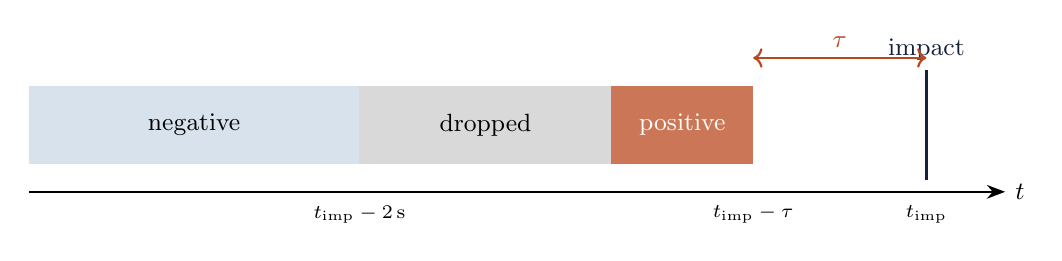
\begin{tikzpicture}[font=\small]
\fill[adlc!18] (0,0) rectangle (4.2,1);          \node at (2.1,0.5) {negative};
\fill[gray!30] (4.2,0) rectangle (7.4,1);        \node at (5.8,0.5) {dropped};
\fill[fallc!75] (7.4,0) rectangle (9.2,1);       \node[white] at (8.3,0.5) {positive};
\draw[very thick,ink] (11.4,-0.2)--(11.4,1.2);   \node[above,ink] at (11.4,1.2) {impact};
\draw[<->,thick,fallc] (9.2,1.35)--(11.4,1.35) node[midway,above] {$\tau$};
\draw[-{Stealth},thick] (0,-0.35)--(12.4,-0.35) node[right] {$t$};
\node[below,font=\scriptsize] at (4.2,-0.4) {$t_{\mathrm{imp}}-2$\,s};
\node[below,font=\scriptsize] at (9.2,-0.4) {$t_{\mathrm{imp}}-\tau$};
\node[below,font=\scriptsize] at (11.4,-0.4) {$t_{\mathrm{imp}}$};
\end{tikzpicture}

\vspace{0.8em}
\begin{columns}[T]
\begin{column}{0.32\textwidth}\small $\tau=0$: window ends on impact, classic \textbf{detection}.\end{column}
\begin{column}{0.32\textwidth}\small $\tau>0$: only the dip and tilt before impact are seen: \textbf{early warning}.\end{column}
\begin{column}{0.32\textwidth}\small 9 lead times (0 to 1.0\,s); about 1\,456 positive vs.\ 78\,545 negative windows (1\,:\,54).\end{column}
\end{columns}
\end{frame}

% ----------------------------------------------------------------------
\begin{frame}{Visualisation: why a simple threshold fails}
\begin{columns}[c]
\begin{column}{0.62\textwidth}
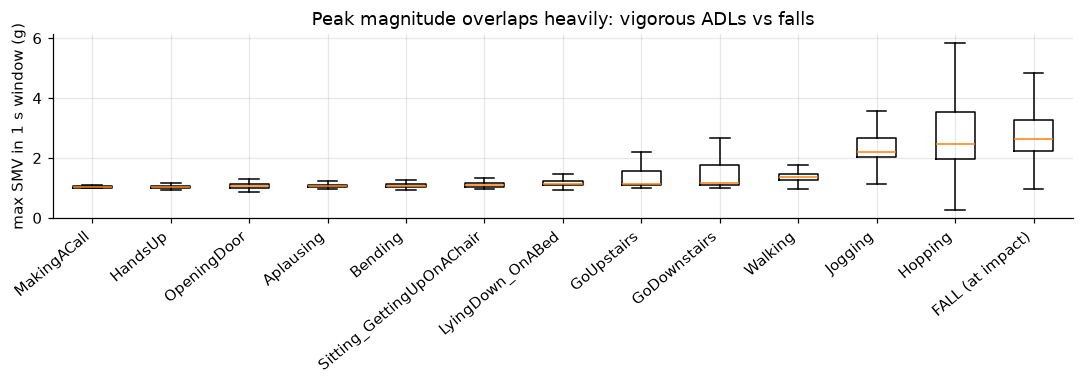
\includegraphics[width=\textwidth]{fig02_peak_overlap.png}
\end{column}
\begin{column}{0.36\textwidth}
\small Jogging and hopping reach peaks as high as a fall: peak size alone cannot separate them.
\end{column}
\end{columns}
\vspace{0.5em}
\begin{center}
\small
\begin{tabular}{lcc}
\toprule
Single rule (ROC-AUC) & $\tau=0$ & $\tau=0.3$\,s\\
\midrule
Peak SMV & 0.652 & \alert{0.479}\\
Free-fall dip & 0.826 & 0.759\\
Tilt change & 0.868 & 0.771\\
\bottomrule
\end{tabular}
\end{center}
\end{frame}

% ----------------------------------------------------------------------
\begin{frame}{Models and why}
\begin{columns}[T]
\begin{column}{0.48\textwidth}
\begin{block}{Three classifiers}
\small
\begin{itemize}
\item \textbf{Logistic regression}: linear, interpretable baseline
\item \textbf{Random forest (main)}: non-linear, robust to noisy features, copes with imbalance; lowest cost at $\tau=0.3$\,s
\item \textbf{Gradient boosting}: strong tabular learner for comparison
\end{itemize}
\end{block}
\end{column}
\begin{column}{0.48\textwidth}
\begin{block}{Validation and decision rule}
\small
\begin{itemize}
\item \textbf{Subject-level 5-fold CV}: nobody is in both train and test, so no memorising of people
\item \textbf{Cost-sensitive threshold}: a missed fall costs 10$\times$ a false alarm; chosen on training folds only (nested), then applied to unseen people
\item Imbalance 1:54: class weights, PR-AUC, recall, false alarms per minute (never plain accuracy)
\end{itemize}
\end{block}
\end{column}
\end{columns}
\end{frame}

% ----------------------------------------------------------------------
\begin{frame}{Results: more lead time makes the problem harder}
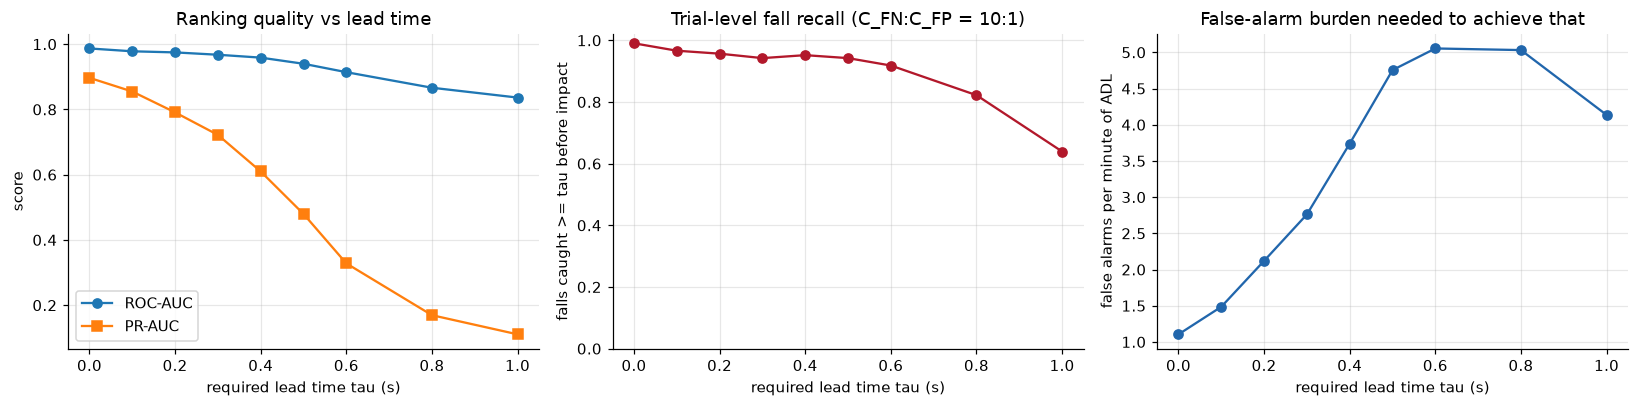
\includegraphics[width=\textwidth]{fig03_tau_tradeoff.png}
\vspace{0.3em}
\begin{center}\small
\begin{tabular}{lccc}
\toprule
 & $\tau=0$ & $\tau=0.3$\,s & $\tau=0.6$\,s\\
\midrule
PR-AUC & 0.90 & 0.72 & 0.33\\
Falls caught (trial level) & 0.99 & 0.94 & 0.92\\
False alarms per minute & 1.1 & 2.8 & 5.1\\
\bottomrule
\end{tabular}
\end{center}
\end{frame}

% ----------------------------------------------------------------------
\begin{frame}{Results: the trade-off between recall and false alarms}
\begin{columns}[c]
\begin{column}{0.5\textwidth}
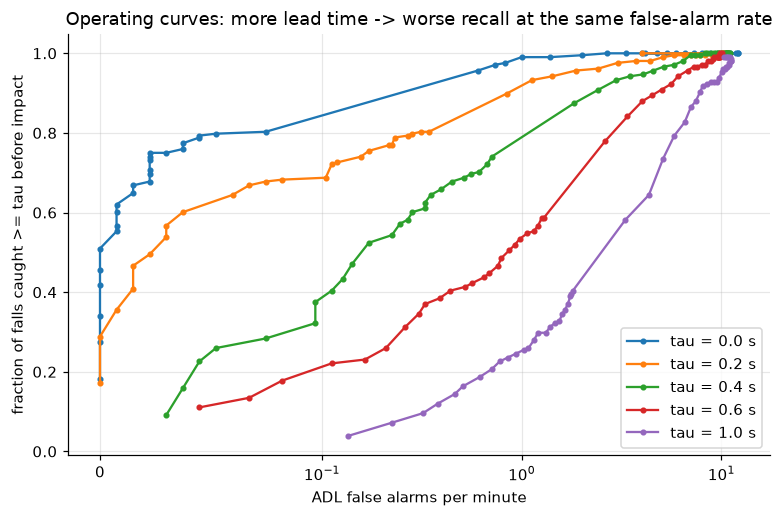
\includegraphics[width=\textwidth]{fig04_operating_curves.png}
\end{column}
\begin{column}{0.48\textwidth}
\small
\begin{tabular}{cccc}
\toprule
$\tau$ (s) & PR-AUC & Falls caught & Alarms/min\\
\midrule
0.0 & 0.90 & 0.99 & 1.1\\
0.2 & 0.79 & 0.96 & 2.1\\
0.4 & 0.61 & 0.95 & 3.7\\
0.6 & 0.33 & 0.92 & 5.1\\
0.8 & 0.17 & 0.82 & 5.0\\
1.0 & 0.11 & 0.64 & 4.1\\
\bottomrule
\end{tabular}
\vspace{0.5em}

Beyond $\approx$0.6\,s even a generous false-alarm budget cannot recover recall.
\end{column}
\end{columns}
\end{frame}

% ----------------------------------------------------------------------
\begin{frame}{Results: the cost ratio sets the operating point}
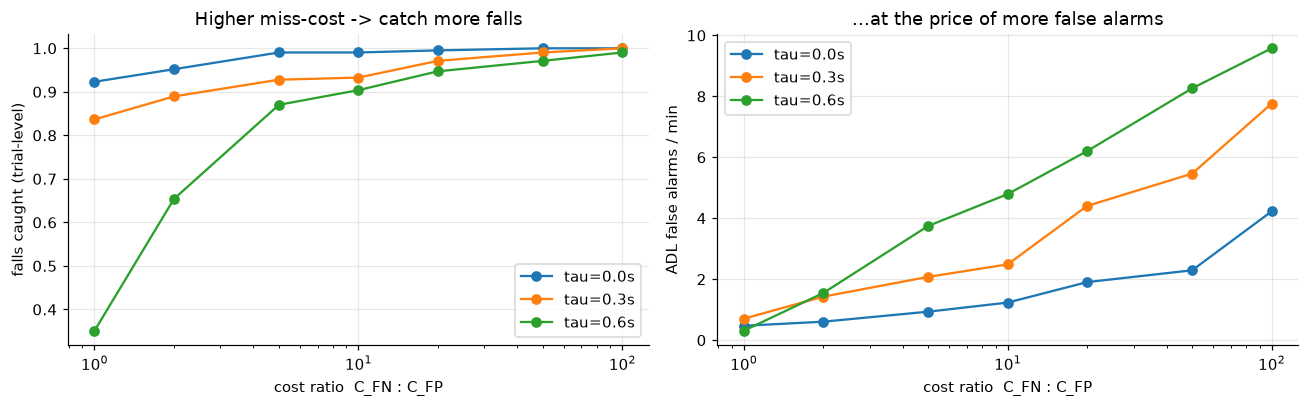
\includegraphics[width=0.88\textwidth,height=0.55\textheight,keepaspectratio]{fig06_cost_sweep.png}
\begin{itemize}\small
\item At $\tau=0.3$\,s: ratio 1:1 catches \alert{84\%} of falls at 0.7 alarms/min; 20:1 catches \alert{97\%} at 4.4; 100:1 catches \alert{100\%} at 7.8.
\item Choose the ratio by application: a hip airbag tolerates false alarms, a robot that stops walking does not.
\end{itemize}
\end{frame}

% ----------------------------------------------------------------------
\begin{frame}{Extension: strict evaluation and temporal persistence}
\begin{columns}[T]
\begin{column}{0.54\textwidth}
\footnotesize
\begin{tabular}{ccccc}
\toprule
$\tau$ & $\Delta$ & Strict recall & Alarms/min & ADL w/ alarm\\
\midrule
0.0 & 0 & 0.971 & 1.21 & 0.277\\
 & 0.4 & 0.962 & 1.21 & 0.272\\
\midrule
0.3 & 0 & 0.913 & 2.46 & 0.508\\
 & 0.2 & 0.899 & 2.41 & 0.490\\
 & 0.4 & 0.899 & 2.48 & 0.501\\
\midrule
0.6 & 0 & 0.894 & 4.91 & 0.814\\
 & 0.2 & 0.846 & 4.32 & 0.771\\
 & 0.4 & \alert{0.817} & \alert{3.72} & 0.717\\
\bottomrule
\end{tabular}
\end{column}
\begin{column}{0.44\textwidth}
\small
\begin{itemize}\setlength\itemsep{0.5em}
\item \textbf{Strict metric:} only alarms in $[t_{\mathrm{imp}}-2\,\mathrm{s},\,t_{\mathrm{imp}}-\tau]$ count; early alarms in fall trials are false alarms.
\item It lowers recall by only \textbf{2--3 points}: the headline result is robust.
\item \textbf{Persistence} ($\Delta$ = mean score over last $\Delta$ s): no effect at 0 and 0.3\,s; at 0.6\,s alarms $-24\%$ but recall $-7.7$ points.
\item A trade-off, not a clear gain: a negative result for short horizons.
\end{itemize}
\end{column}
\end{columns}
\end{frame}

% ----------------------------------------------------------------------
\begin{frame}{Model comparison and feature importance ($\tau=0.3$\,s)}
\begin{columns}[c]
\begin{column}{0.56\textwidth}
\small
\begin{tabular}{lcccc}
\toprule
Model & ROC & PR & Cost & Alarms/min\\
\midrule
Logistic reg. & 0.941 & 0.472 & 5714 & 3.70\\
\alert{Random forest} & \alert{0.968} & \alert{0.722} & \alert{4156} & \alert{2.76}\\
Grad.\ boosting & 0.960 & 0.710 & 4454 & 3.95\\
\bottomrule
\end{tabular}
\vspace{0.7em}

\small Top features: window mean SMV, dip depth, min SMV in the last 0.5\,s, std of the previous second: a drop below the preceding level after a calm period.
\end{column}
\begin{column}{0.4\textwidth}
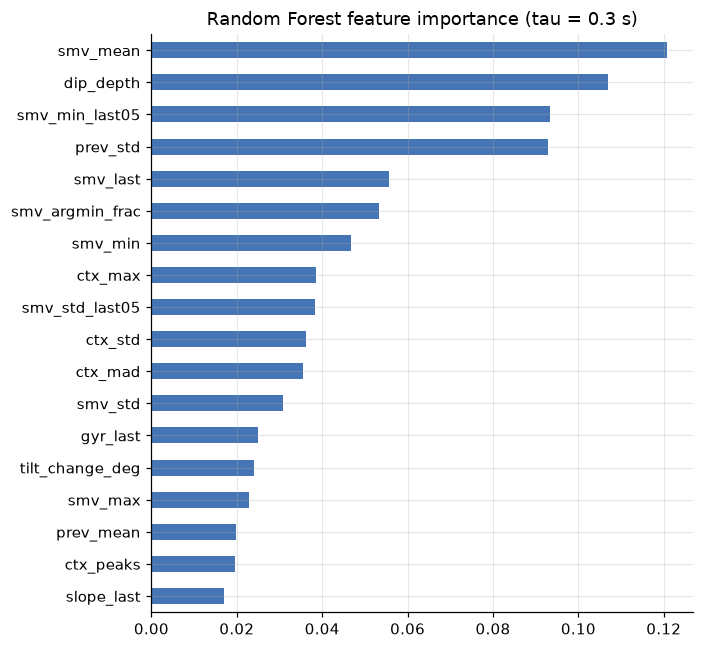
\includegraphics[width=\textwidth,height=0.75\textheight,keepaspectratio]{fig05_feature_importance.png}
\end{column}
\end{columns}
\end{frame}

% ----------------------------------------------------------------------
\begin{frame}{Which sensor position works best? ($\tau=0.3$\,s, accelerometer only)}
\begin{columns}[c]
\begin{column}{0.55\textwidth}
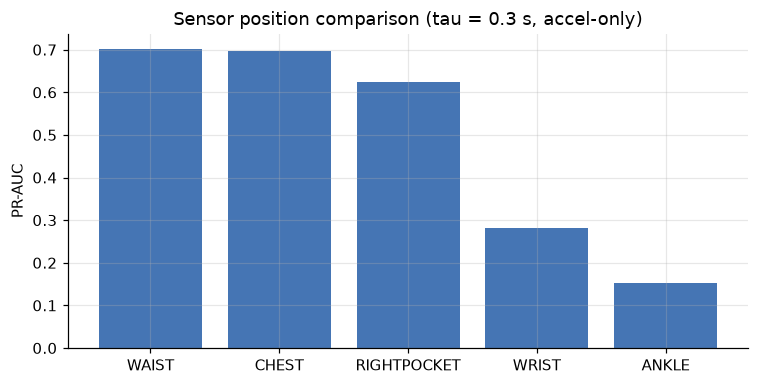
\includegraphics[width=\textwidth]{fig07_positions.png}
\end{column}
\begin{column}{0.43\textwidth}
\small
\begin{tabular}{lcc}
\toprule
Position & PR-AUC & Alarms/min\\
\midrule
Waist & 0.701 & 3.18\\
Chest & 0.698 & 2.85\\
Pocket & 0.623 & 3.74\\
Wrist & 0.282 & 6.05\\
Ankle & 0.152 & 4.60\\
\bottomrule
\end{tabular}
\end{column}
\end{columns}
\vspace{0.5em}
\begin{itemize}\small
\item Chest and waist (near the centre of mass) are best; a phone in the pocket loses little.
\item Wrist and ankle lose most of the signal: limb motion is dominated by other activities.
\end{itemize}
\end{frame}

% ----------------------------------------------------------------------
\begin{frame}{Error analysis ($\tau=0.3$\,s)}
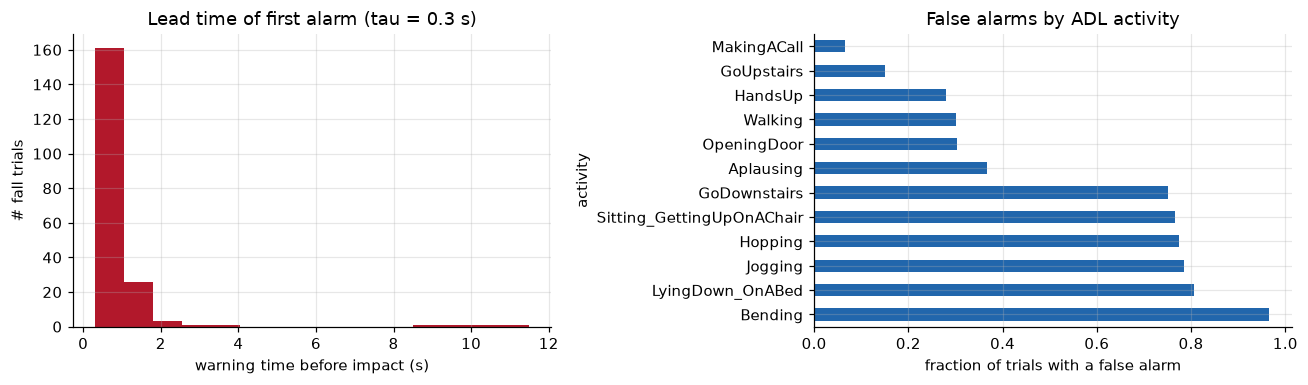
\includegraphics[width=0.92\textwidth,height=0.5\textheight,keepaspectratio]{fig08_error_analysis.png}
\begin{itemize}\small
\item Falls caught by type: backward 96\%, forward 94\%, lateral 92\%.
\item Most false alarms: bending (97\% of trials), lying down (81\%), jogging (79\%), hopping (77\%), sitting/getting up (77\%).
\item Fewest: making a call (7\%), going upstairs (15\%), hands up (28\%), walking (30\%).
\end{itemize}
\end{frame}

% ----------------------------------------------------------------------
\begin{frame}{Limitations and honest caveats}
\small
\begin{columns}[T]
\begin{column}{0.49\textwidth}
\begin{itemize}\setlength\itemsep{0.5em}
\item Falls are \alert{simulated} by young, healthy volunteers; elderly falls differ.
\item Only 19 subjects; one subject has 56 of the 208 falls; single seed, no confidence intervals.
\item 20\,Hz sampling: the dip is resolved only to 50\,ms.
\end{itemize}
\end{column}
\begin{column}{0.49\textwidth}
\begin{itemize}\setlength\itemsep{0.5em}
\item Impact = peak SMV: wrong for a few suspicious trials.
\item \alert{False-alarm burden is high:} at $\tau=0.3$\,s, 55\% of ADL trials raise at least one alarm.
\item Trial-level recall counts any alarm before $t_{\mathrm{imp}}-\tau$ (0.94 vs.\ window-level 0.80 at $\tau=0.3$\,s); the strict metric lowers it by only 2--3 points.
\end{itemize}
\end{column}
\end{columns}
\end{frame}

% ----------------------------------------------------------------------
\begin{frame}{Conclusions and future work}
\begin{enumerate}\setlength\itemsep{0.7em}
\item Falls leave an early physical signature (free-fall dip and tilt) that a classifier can use before impact.
\item Early warning is a trade-off: at $\tau=0.6$\,s PR-AUC falls from 0.90 to 0.33 and false alarms rise from 1.1 to 5.1 per minute.
\item The cost ratio lets the application choose its operating point; chest and waist sensors work best, wrist and ankle lose much.
\item Strict evaluation changes recall by only 2--3 points; temporal persistence reduces false alarms only at 0.6\,s, and at a cost in recall.
\end{enumerate}
\vspace{0.5em}
\begin{block}{Future work}
\small Orientation-corrected features (magnetometer), sequence models (1-D CNN / LSTM), fusion of several positions, personalised thresholds, other datasets (e.g.\ SisFall) and data from older adults.
\end{block}
\end{frame}

\begin{frame}[plain]
\centering
\vspace{2.5cm}
{\Huge Thank you}\\[0.8em]
\end{frame}

\end{document}
